\documentclass[fleqn, 14pt]{extarticlej}
\oddsidemargin=-1cm
\usepackage[dvipdfm]{graphicx}
\textwidth=18cm
\textheight=23cm
\topmargin=0cm
\headheight=1cm
\headsep=0cm
\footskip=1cm

\def\labelenumi{(\theenumi)}
\def\theenumii{\Alph{enumii}}
\def\theenumiii{(\alph{enumiii})}
\usepackage{comment}
\usepackage{indentfirst}
\usepackage{float}
\begin{document}
%%%%%%%%%%%%%%%%%%%%%%%%%%%%
%% 表題
%%%%%%%%%%%%%%%%%%%%%%%%%%%%
\begin{center}
{\Large {\bf EnCalのモデルを扱う機能の提案}}

\end{center}
\begin{flushright}
2013年6月13日

乃村研究室 河野 達生
\end{flushright}
%%%%%%%%%%%%%%%%%%%%%%%%%%%%
%% はじめに
%%%%%%%%%%%%%%%%%%%%%%%%%%%%
\section{はじめに}
自身の研究テーマは,「情報の可視化,整理」である.このため,EnCalで用いられるモデルの可視化,整理を行う.EnCalとは,作業発生の規則性を扱うカレンダシステムである[1].EnCalでは,作業発生の規則性を表すモデルとしてMissionやRecurrenceが存在する.Missionとは,TaskまたはMissionを要素とする集合である.Recurrenceとは,繰り返し発生する同様のTaskを1つの集合である.Taskとは,作業を扱う最小の単位である.本資料は,これらのモデルを効率良く見つけ,作成する
方法を提案する.

\section{Recurrence,Missionの作成}
\subsection{現在のEnCalのUI}
現在のEnCalのUserInterface(以下UIとする) を図1に示す.EnCalのUIは,以下の4つから構成されている.
\begin{enumerate}
	\item 主として操作するカレンダ\\
	主として操作するカレンダは,Taskを登録できる.また,MissionsやEvent Forecastingからドラッグアンドドロップすることで,Taskを登録できる.
	\item 過去のカレンダ\\
	過去のカレンダは,主として操作するカレンダと同様の機能をもつ.過去のカレンダに登録されているTaskを主として操作するカレンダにドラッグアンドドロップすることで,Taskを登録できる.
	\item Missions\\
	Missionsは,関連性をもつTaskをまとめたMissionsの一覧である.
	\item Event Forecasting\\
	Event Forecastingは,予測されたTaskの一覧である.

\end{enumerate}

\begin{figure}[h]
  \begin{center}
    \includegraphics[clip,width=1\columnwidth]{zu3.eps}
    \caption{現在のEnCalのUI}
  \end{center}
\end{figure}

\subsection{Missionの作成}
現在のEnCalのUIにおいて,Missionは,主として操作するカレンダや過去のカレンダに存在するTaskをMissionsへドラッグアンドドロップすることで作成される.Missionsの表示は,主として操作するカレンダ月に依存するものとなっている.このため,過去のMissionを探し出す場合,ユーザは日付を把握し,カレンダの月を移動する必要がある.\\

\subsection{Recurrenceの作成}
現在のEnCalのUIにおいて,Recurrenceは,Taskを主として操作するカレンダから過去のカレンダにドラッグアンドドロップする,または,Taskを過去のカレンダから主として操作するカレンダにドラッグアンドドロップすることで作成される.Recurrenceは,カレンダ上に表示されていない.Taskの詳細において,Recurrenceに含まれるTaskの一覧を確認できる.\\

% \begin{enumerate}
% 	\item 目的の達成\\
% 情報を探す際,ユーザの目的が達成できるUIにする必要がある.リンクの名前やページの見出しにこのページの概要を記述する.
	
% 	\item 注意を引くフォント\\
% 	ユーザの注意を引くフォントにする必要がある.作者の最も伝えたい部分のフォントの大きさ,色,及び書体を変更する.
	
% 	\item 独自機能の排除\\
% 	独自の機能は排除する必要がある.独自の機能を追加していることで,ユーザは使い方を理解できない可能性がある.
	
% 	\item 形式の統一\\
% 	ページ内の形式を統一する必要がある.統一することで,ユーザの理解を早めることができる.

% \end{enumerate}

\section{機能案}
MissionやRecurrenceを効率良く見つける,または作成するためには,Taskをどのように表示するかが重要である.本資料では,以下の3つの機能を提案した.\\
\begin{enumerate}
	\item Taskの一覧\\
	Taskの一覧を表示させる機能を提案する.これにより,月に依存せずにTaskを確認でき,MissionやRecurrenceを作成できる.
	\item Taskのソート
	\begin{enumerate}
		\item 名前順にソート\\
		Taskの一覧の機能から,名前順にソートを行う機能を提案する.MissionやRecurrenceを作成する際,ユーザが同様のTaskから別のMissionやRecurrenceを作成している場合がある.これにより同様のMissionやRecurrenceが作成され,数が増えてしまう問題が起こる.ソートを行い整理することで,この問題を防ぐ.図2に,Taskを名前順にソートした例を示す.
	
\begin{figure}[h]
  \begin{center}
    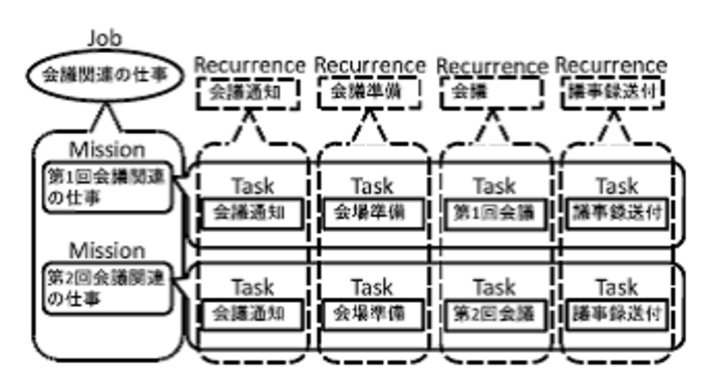
\includegraphics[clip,width=0.8\columnwidth]{zu1.eps}
    \caption{名前順にソートの例}
  \end{center}
\end{figure}
	
		\item 繰返しの回数順にソート\\
			Taskの繰返しの回数順にソートを行う機能を提案する.これにより,Taskの発生回数を把握ができる.発生回数が同じTaskから,新たなMissionやRecurrenceを見つけられると考えられる.図3に,Taskを繰返し回数順にソートした例を示す.
	\end{enumerate}
	
\begin{figure}[h]
  \begin{center}
    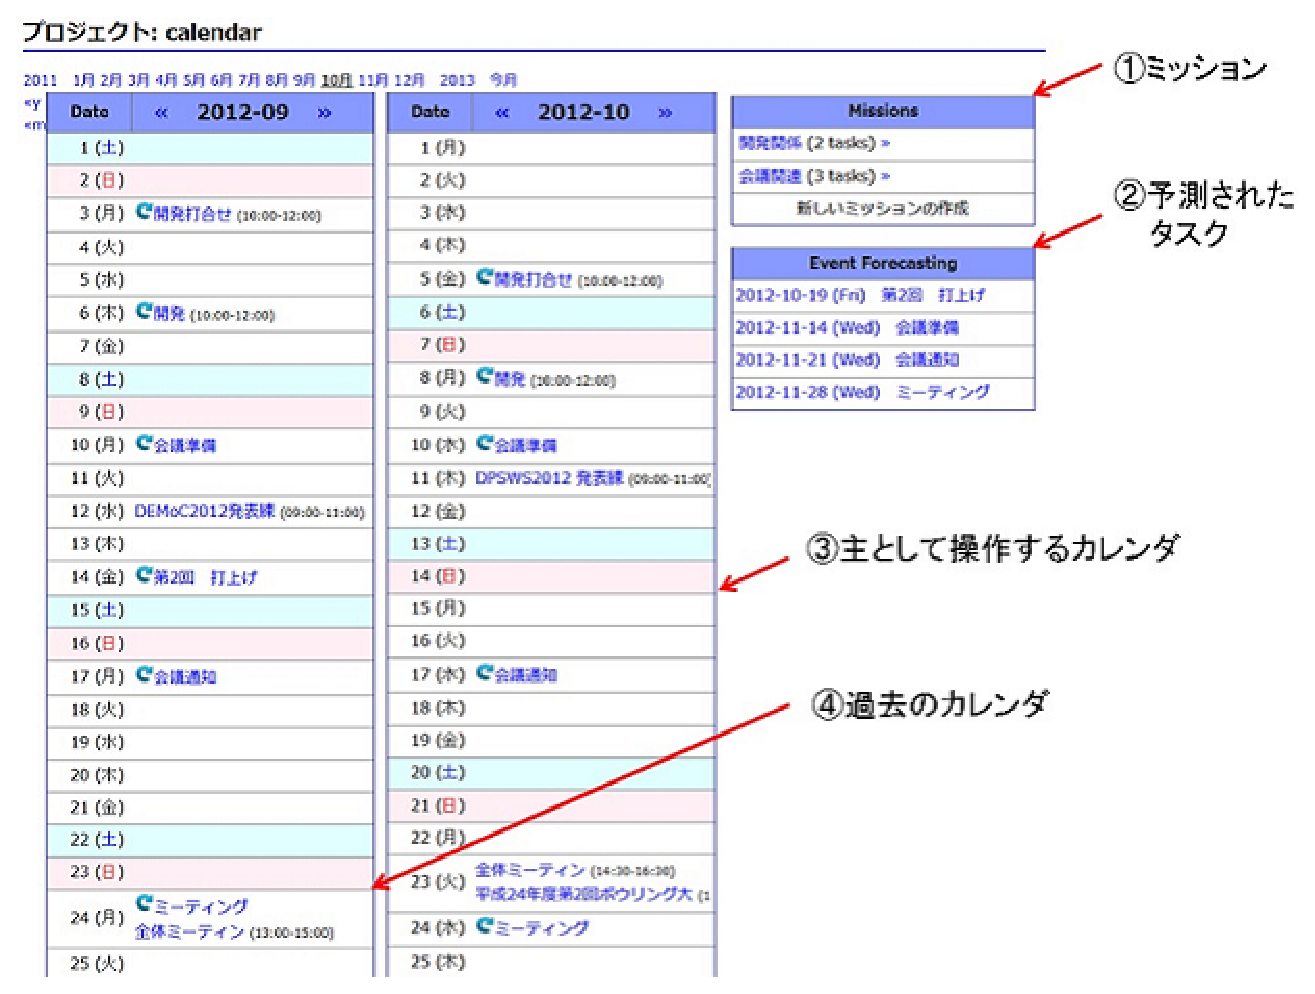
\includegraphics[clip,width=0.8\columnwidth]{zu2.eps}
    \caption{繰返し回数順にソートの例}
  \end{center}
\end{figure}
	
	\item Taskの検索\\
	Taskを検索する機能を提案する.必要なTask見つけ出す際,一覧の中から探すのは手間である.検索機能を追加することで,この問題を防ぐことができる.
	
\end{enumerate}

\newpage
\section{考察}
UIに対する感じ方は,人によって異なるため,「情報の可視化,整理」について,さらなる検討の余地がある.このため,本資料で提案したMissionやRecurrenceのモデルを扱う方法だけでは,十分ではないと考える.今後,上記の機能を実装した上で,再び考察を行う必要があると考える.

\begin{thebibliography}{99}
	\bibitem {book1}
三原俊介,谷口秀夫,乃村能成,南裕也:作業発生の規則性を扱うカレンダシステムの評価,情報処理学会論文誌,Vol.540,No.2,pp.630-638(2013).
\end{thebibliography}

\end{document}
